%!TEX root = ../thesis.tex
%*******************************************************************************
%*********************************** First Chapter *****************************
%*******************************************************************************

\chapter{Introduction}  %Title of the First Chapter
\label{chapter1}

\graphicspath{{Chapter1/figs/}}

Machine Learning (ML) has positioned itself as a hot topic and almost as a synonym to Data Analysis (DA). This misconception can be dangerous when domain-expert, data scientists, statisticians or even public in general try to extract valuable knowledge from a dataset. Both concepts are yet continuously evolving, therefore the first effort consists of establishing a common definition aligned with the contributions presented in this work. 

DA intend to seek through a dataset for interesting relationships and information and to effectively present them as insights \cite{TukeyJohnW.andWilk1966DataOverview}. More specifically, Exploratory Data Analysis (EDA) is a systematic way to investigate relevant information from multiple perspectives and it is not fixed to a set of techniques \cite{Yu2003ExploratoryAnalysis}. By the other hand, ML does comprises a set of techniques enabling computers to learn from experience and automatically to improve their efficiency \cite{Michie1968MemoLearning} without being explicitly programmed \cite{Koza1996}. When it is tedious or even impossible to detect patterns in larger and high-dimensional datasets, ML provides mechanisms to explore alternate routes to understand the data \cite{Yu2003ExploratoryAnalysis}. Commonly, EDA user tasks can involved actions for search or query information in terms of groups, outliers, distributions, correlations, among others \cite{Munzner2014VisualizationDesign}. From the most classical ML perspective, these tasks can be achieved applying supervised Classification and Regression algorithms, where labels drive the learning process, or Dimensionality Reduction (DR) or Clustering algorithms when data patterns or structures need to be discovered. It is important to note that the ML process is automated, so the user is responsible for checking its results and decide if these fit to a schema, mental model \cite{Grolemund2014AAnalysis}, representing the real-world phenomenon evidenced in the data.

%, when it is not possible to have access to data labels or these does not match with the real-world phenomenon to represent.

ML techniques, being black-boxes working autonomously, have currently two big problems for the EDA purposes: 

\begin{enumerate}
\item Lack of user feedback. To be an iterative process, training ML models can require a lot of execution time for achieving acceptable results and, in the worst case, these can be completely useless. If the user is a domain-expert, their knowledge about the problem could greatly improve the overall performance of the ML model in less amount of time.
\item More sophisticated models support the accomplishment of complex tasks but generally losing interpretability. When user is involved in the ML process, model performance could not be the unique requirement to be fulfilled. While the ML objective might be to reduce error, the real-world purpose is to provide useful information \cite{Lipton2017} for decision-making by the user. The practice of handing over human judgment to the computer when user does not understand how this is working, it is similar to blindly accept that two datasets are comparable when having the same measures of central tendency.
\end{enumerate}

To address this, two new sub-fields of research have been proposed to help users to better interact and understand ML models, and by this opening the black-box: Interactive ML and Interpretable ML (also known as Explainable AI). In this work, a selection of the most noteworthy papers of these sub-fields are presented and some guidelines for designing better and more user-centric ML systems are derived. Subsequently, this analysis focuses on Visual Analytics (VA) tools for exploring high-dimensional data that use DR or Clustering algorithms.

From the previous basis, a web interactive tool for exploring high-dimensional tabular data is developed extending the concept that ML models can be used for gaining data understanding as long as the user is able to feed them by interactions and interpret their inner workings and results. For supporting the exploration, two implementations \cite{Pezzotti2018LinearWeb},\cite{Asensio2018Ml-kmeans} of the t-SNE and K-Means algorithms running in the browser are integrated. Opportunities in a browser-based environment include shareability, interactivity and on-device computation \cite{Smilkov2019TensorFlow.js:Beyond}. This tool is intended to be used by domain-expert users where these are able to interactively load their own dataset, perform attribute selection and instance filtering, train the available models, change their hyper-parameters and validate their results. The tool evaluation is performed by two real-world use cases where domain-expert users are asked to explore the data by cluster-oriented DR task sequences \cite{Brehmer2014VisualizingSequences} and extract insights.

%********************************** %First Section  **************************************
\section{Motivation examples} %Section - 1.1 
\label{section1.1}

No extending the discussion about different statistical or VA alternatives for analyzing high-dimensional data, two idioms for visualizing it are parallel coordinates and scatter plot matrix. Both idioms are useful for determine correlations between attribute pairs and identify outliers but, particularly the parallel coordinates, presents a limitation when analyzing non-neighbor attributes in terms of their distribution among the x-axis. These idioms can be extended by including user interaction for linked highlighting across sub-views, for the case of the scatter plot matrix, or attribute reordering, seeking to reduce the parallel coordinates limitation previously presented.

Figures \ref{fig:iris-parallel} and \ref{fig:iris-scatterplot} shows these idioms applied to one the most widespread datasets in ML community, the Fisher's Iris dataset \cite{FisherIris} which has 150 items, 4 attributes and one class representing the iris species. In both idioms, the main insight from this dataset consisting of the class linear separability in two of the attributes (PetalLengthCm, PetalWidthCm) can be easily appreciated.

\begin{figure}[ht]
 \centering
 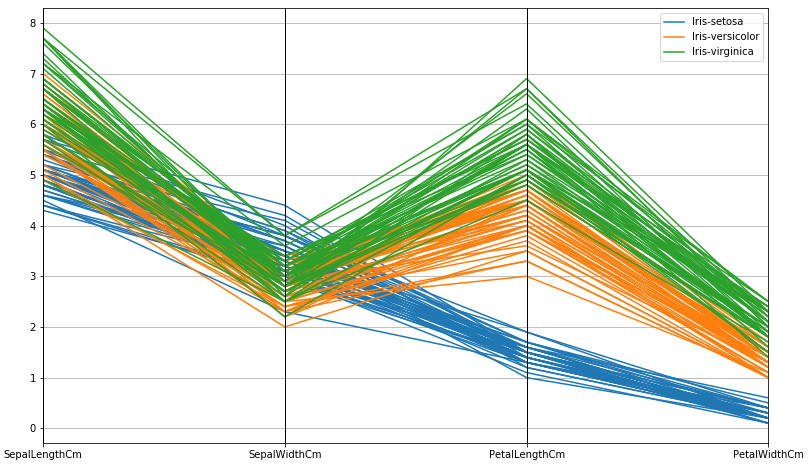
\includegraphics[width=0.7\textwidth]{iris-parallel.png}
 \caption{Parallel coordinates for the Iris dataset \cite{FisherIris}}
 \label{fig:iris-parallel}
\end{figure}

\begin{figure}[ht]
 \centering
 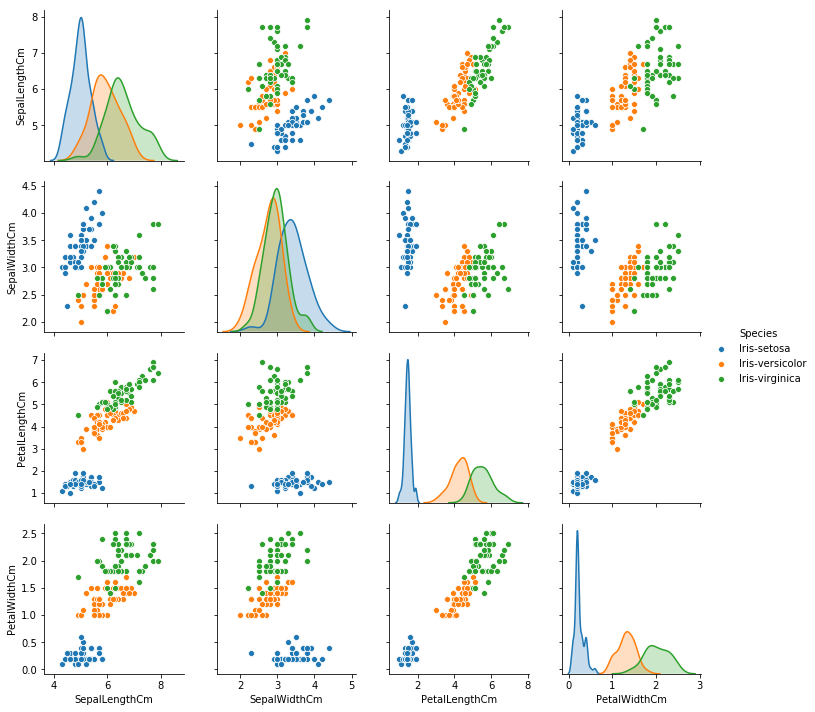
\includegraphics[width=0.9\textwidth]{iris-scatterplot.png}
 \caption{Scatter plot matrix for the Iris dataset \cite{FisherIris}}
 \label{fig:iris-scatterplot}
\end{figure}

In the real-world, there are larger and more complex datasets than the Iris having hundreds of attributes and thousands or millions of items. For most of these cases, using the previous idioms is ineffective given the user cognition constraints for retaining many details, even when they are all shown at the same time, in addition to the screen size constraint. Next subsections describe two datasets considered relevant for this study and a possible exploratory analysis path supported by ML DR and Clustering algorithms.

\subsection{The FIFA 19 Complete Player dataset} %Subsection - 1.1.1 
\label{subsection1.1.1}

FIFA

\subsection{The SALURBAL dataset} %Subsection - 1.1.2 
\label{subsection1.1.2}

SALURBAL

%********************************** %First Section  **************************************
\section{Document structure} %Section - 1.2 
\label{section1.2}

This document is organized as follows: Chapter \ref{chapter2} shows the state of the art analysis for the Interactive ML and Interpretable ML sub-fields and the first contribution in terms of the guidelines for designing better and more user-centric ML systems. Chapter \ref{chapter3} describes some traditional DR and Clustering algorithms and discuss the current advances for interact and interpret them. Chapter \ref{chapter4} presents the web interactive tool for exploring high-dimensional tabular data supported by DR and Clustering models. Chapter \ref{chapter5} evidences the results of the tool evaluation based on two real-world case studies. Finally, Chapter \ref{chapter6} concludes the work and presents the challenges and opportunities for the future.